\documentclass{article}
\usepackage[utf8]{inputenc}

\title{Spatio-temporal prediction of NO2 in Madrid, Spain}
\author{Meng Lu}
\date{October 2017}

\usepackage{natbib}
\usepackage{graphicx}
\usepackage{cleveref}
\usepackage{booktabs}
\usepackage{todonotes}


\begin{document}

\maketitle


\section{Introduction}

The number of air quality measurement stations is often limited to
quantify air pollution continuously in space and time. Other data
sources such as physical and chemical model simulations and
spatiotemporal correlations may play an important role in improving
air pollution interpolation. In this study, we investigated different
spatio-temporal and non-spatio-temporal statistical models and
integrated historical records and predictions from numerical
physi-chemical model simulations to station measurements to predict
air quality pollution.

We compared the results of air prediction from linear and non-linear
regression models, geostatistical models, and random forest
models. The linear and non-linear regression models assume no spatial
correlation and purely predict using the CAMS/MACC model
simulations. We consider an ordinary kriging and an universal kriging
model to integrate spatial correlation and predict air pollution. For
each linear/nonlinear regression, geostatistical, and random forest
models, we attempted different methods and attempted to achieve the
best results from these models.

The objective is to find the best prediction method with the available
data. The objective is guided by three research questions:
\begin{itemize}
\item Can spatial correlation between a limited number of air quality
  measurement stations be used to improve air quality prediction?
\item Can the CAMS/MACC model predictions improve local air quality
  predictions?
\item How can we construct an integrated model to predict air
  quality with station measurements, MACC simulation, and temporal
  variables? Does the inclusion of time series characters, such as
  trend and harmonic terms improve model prediction?
\end{itemize}

\section{Data}
\label{sec:data}

Three years of hourly NO2 station measurements and CAMS/MACC
simulations are available. There are in total 24 stations distributed
in the city of Madrid, Spain. These station measurements are used to
to train models and to validate the modeling results.  \todo{Add a
  deeper description of the data (JLA).}

The distribution of CAMS/MACC forecast of NO2 is very close to
Gaussian. The distribution of the measured NO2 is a skewed Gaussian
distribution with mean around 33.\todo{Add a graph of both
  distributions. It is weird, however, that they are so different (one
  skewed, one not).}


\section{Forecasting methods}

We consider a variety of linear, non-linear regression models,
ordinary and universal kriging methods, and random forest methods to
predict NO2 spatiotemporally. Each of these methods are described in
detail.

The NO2 predicting methods considered and compared are:
\begin{enumerate}
    \item Ordinary kriging of CAMS/MACC simulation
    \item Linear regression model with CAMS/MACC, harmonic terms and
      time of day (TOD) as potential independent variables.
    \item Polynomial and GAM (general additive model) with CAMS/MACC
      as independent variables.
    \item Universal Kriging with CAMS/MACC simulation and potentially
      coordinates as variable.
    \item Random forest prediction with CAMS/MACC and different
      temporal variables.
\end{enumerate}

\subsection{Interpolation of CAMS/MACC simulation \todo{Title should be
  coherent with the previous enumeration of models.} } 
The CAMS/MACC simulations show strong spatial correlation. In order to
assimilate more information from historical CAMS/MACC numerical
predictions, we computed a pooled variogram from CAMS/MACC forecasts
of 200 sampled time stamps. The variogram is automatically fitted with
the initial parameters of nugget, sill and range set as
\citet{automap}. An Ste (Matern, M. Stein’s parameterization \todo{Add
  cite to Matern \&c.}) model is used to interpolate CAMS/MACC
forecasts to the city grid and to each of the measuring stations.

\subsection{Linear regression model with CAMS/MACC as an independent variable.}

The models in this section investigate linear or non-linear
relationship between MACC simulation and station measurements. Linear,
polynomial, and general additive models are attempted. (Adjusted) R
square and model complexity were considered in model selection.
  
Five models are attempted to investigate the relationship between
station measurements and spatially interpolated CAMS/MACC
forecast. Model 2a and 2b are linear regression models. In model 2b,
TOD (time of day) and harmonic terms are used as additional
independent variables. The models are built with station measurements
and corresponding CAMS/MACC simulations from 2012-01-01 to 2015-12-31
(table 1).

The harmonic terms $|sin(2 \pi wt) + \phi|$, with
$w = 1 / (356 * 2 * 2)$ are used to fit the half year positive
cyclical pattern\todo{It would be nice to justify this
  graphically.}. 45\% percent of variance could be explained by this
model ($lm (station measurements \sim MACC + |sin(a)| + |cos(a)|)$
\todo{This formula is not clear. What is $a$? What is $lm$?}).

\begin{table}[tbp]
\centering
\begin{tabular}{ c c c }
  \toprule
Model & Method & Independent variable\\ \midrule

2a &linear regression & MACC   \\
2b &linear regression & MACC, TOD, Harmonics   \\
2c1 & second order polynomial & MACC \\  
2c2 & third order polynomial & MACC   \\ 
2d & general additive model & MACC  \\  \bottomrule
\end{tabular}
\caption{ Linear and non-linear regression models and the independent variables of the model. TOD: time of day. Harmonics: $ | sin(a)| + |cos(a)|$ } 
\label{table:1}
\end{table}

\begin{figure}[tbp]
  \center
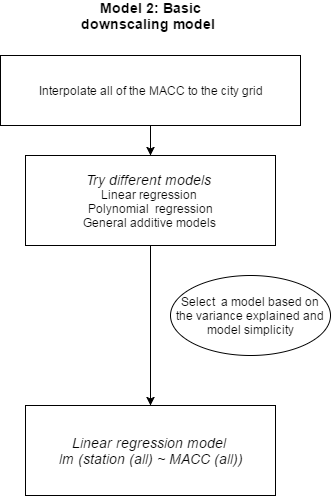
\includegraphics[scale = 0.4]{diaM2.png}
\caption{The workflow of model 2. The model 2a, which is a linear
  regression model with MACC as independent variable has recieved the
  best results and used to compare with models using other methods. }
\label{fig:LR}
\end{figure}

\todo[inline]{A question rises when reading Table \ref{table:1}: why
  we didn't use the TOD and the harmonics in 2c1, 2c2 and 2d? And why
  didn't we use the day of the week (DOW) and day of the year (DOY)
  variables? It is known that the NO2 series shows a weekly and yearly
  cycle. We should be prepared to answer it in revision phase (or
  solve it beforehand).}

\subsection{Universal Kriging}
The basic downscaling models do not utilise spatial information. We
attempted with Universal Kriging to utilise spatial correlations.  Two
models are attempted: 1) with residual variograms with MACC
simulations as a regressor, and 2) with residual variograms with MACC
simulations and locations as regressors.

We sampled 300 time stamps, compute a pooled variogram (average over
the semivariance of each time stamp).

\subsubsection{Manually fitting a variogram model to the variogram}
As no spatial correlation is revealed in the variogram\todo{add a 3D
  graph of the variogram.}, fitting a variogram model automatically to
it is not useful. We define the sill and nugget of a variogram model
to fit to the variogram, then apply universal kriging using this
variogram model to interpolate station measurements to the city grid
and forecast to the next halfday.

\subsubsection{Universal kriging models}

\begin{figure}[tbp]
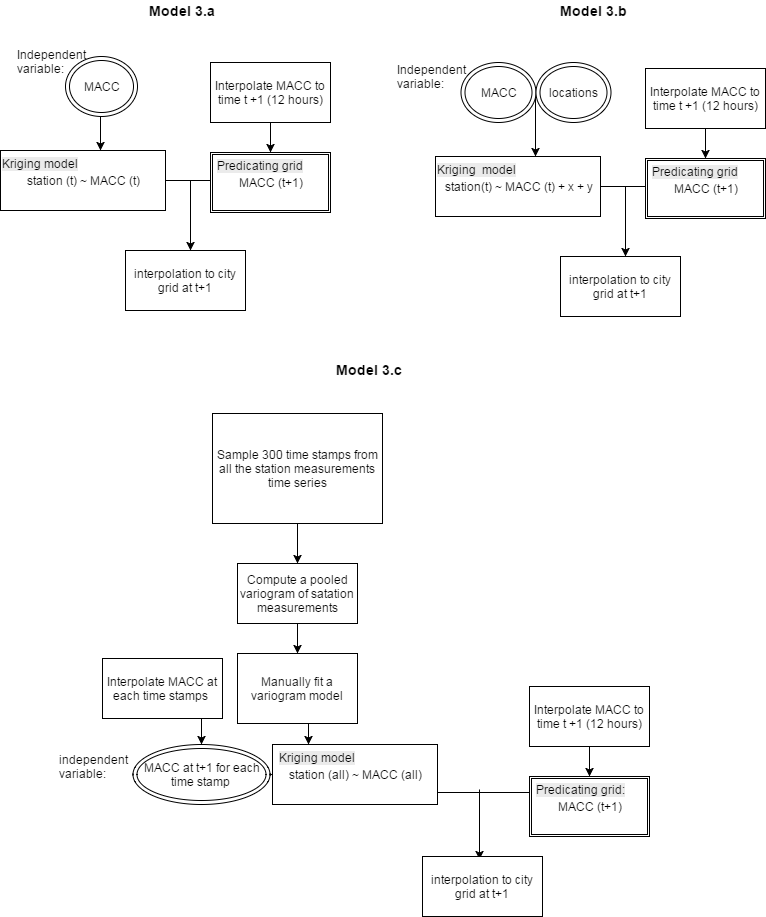
\includegraphics[width=\columnwidth]{diaM3.png}
\caption{Flowchart for the universal krigging models. Model 3a: using
  station measurements and MACC simulations at the same time to fit a
  model, then using MACC simulations at time t+1 to predict. Model 3b:
  Using station measurements and MACC simulations at the same time, as
  well as locaitons to fit a model, then using MACC simulations at
  time t+1 as well as locations to predict. Model 3c: Using all the
  measurements (about 4 years of halfday data) to fit a linear
  regression model, then apply universal Kriging with fixed
  coefficients from the linear regression model. The model is applied
  to the MACC simulations at time t+1 to predict air quality.}
\label{fig:UK}
\end{figure}

Figure \ref{fig:UK} \todo{I believe it's better to have the 3 diagrams
  in different figures.} shows the workflow the model 3a-c. The first
two models (3a and 3b) use spatial data from the most recent time
stamp to fit the data. The drawback of these two models is that the
measurements or MACC forecasts at one or more stations may strongly
affect the linear regression model (i.e. the relationship between MACC
forecasts and station measurements may be inverted). These models 3a
and 3b are more suitable to the situation that more stations
(e.g. more than 100) are available or when there is a lack of
historical time series data. In this study, we used data from all the
locations and times to fit the linear regression model, and applied
Kriging to the linear regression model residuals.

\todo[inline]{I think we will have to make this section more detailed,
stressing the justification for the decisions we made.}

 
\subsubsection{Residual variogram} 

The residual variogram of a linear regression model with MACC
simulations as a regressor.  It could be observed that the spatial
correlation is not revealed from the 24 station measurements. Three
possible reasons are: 1) there are too few observations (stations), 2)
there is a lack of information from short-distance placed stations, 3)
due to the design of the air pollution measuring station network, the
stations are placed where the pollution is suspected to be high, e.g.,
near factories, in a canyon.  distance semivariance
 
\todo[inline]{I think we will have to make this section more detailed,
stressing the justification for the decisions we made and graphs
showing the lack of spatial correlation.}

\subsubsection{Pooled variogram}

Pooled variogram is computed from spatiotemporal points, which uses
more information than only using data from a time stamp and reduces
the influence of extreme values.  Firstly we sample 300 time stamps
that contain no missing data. Then, we compute a pooled residual
variogram (average semivariance) of (1) a linear regression model with
CAMS/MACC simulations as a regressor, and (2) a linear regression
model with CAMS/MACC simulations as a regressor. \todo{This is a
  mistake: (1) and (2) are the same.}

The pooled residual variogram with CAMS/MACC as independent variables
(figure 5\todo{Figure 5 is unexistent.}) contains a little more
information than the variogram of a time stamp. Still, spatial
correlation is not shown in the pooled variogram. The pooled residual
variogram (figure 6\todo{Missing figure.}) with CAMS/MACC and
locations as independent variables also does not reveal spatial
correlation.

\todo[inline]{What are the consequences and implications of the
  findings in this section? I think we should expand.}

\subsection{Random forest}

\begin{table}[tbp]
\centering
\begin{tabular}{ c c  }
Model &  Independent variable\\ \hline 

 4.1 & MACC simulations, DOY, harmonic term, TOD \\
 4.2a & MACC simulations, DOY, TOD (factors) \\
 4.2b & MACC simulations, DOY (factors), TOD (factors) \\ 
 4.3 & DOY, MACC simulations \\
 4.4 & MACC simulations  \\  \hline
\end{tabular}
\caption{Independent variables used in each model. DOY: day of year, TOD: time of day  } 
\label{table:rf}
\end{table}

At last, we used a machine learning method to find a relationship
between NO2 station measurements, MACC simulation, and other temporal
variables. Specipically, we used MACC simulation, day of year (DOY),
time of day (TOD), lagged MACC simulations and harmonic terms as
independent variables in the random forest models.

The R package \texttt{ranger} is used to perform random forest. In
this study, it is found that \texttt{ranger} is faster than the
\texttt{randomForest} package. \todo{Depending on the journal,
  implementation details are better off in a final appendix.}

Table \ref{table:rf} shows the variables that are used in each
model. The harmonic term that is used in model 2
($|sin(2 \pi wt) + \phi|$) is used in the one of the random forest
model. The differences between model 4.2a and model 4.2b is that the
model 4.2b treats DOY as factors while model 4.2a treats it as
numbers. As using a lagged MACC (as is used for Ozone) to forecast
Ozone obtains the lowest accuracy, and is slow, for NO2 this model is
taken off. \todo{The reference to ozone is not clear here (so far only
  NO2 is mentioned.}

\todo[inline]{In this section it is not very clear how did we use the
  spatial information, if we did at all. A diagram would be useful.}


 

\section{Accuracy assessment}

The first half of the data (i.e. the first 1.5 years of time series,
in total 1420 observations) are used to train the forest. The second
half of the data (i.e. the last 1.5 years of time series, in total
1428 observations) are used to test the model. The missing values are
filled using spline interpolation. \todo{Missing values should be
  dealt with in Section \ref{sec:data}.}  The error of Model 3c is
assessed different from other models, as spatial errors are
assessed. It is not feasible to compare station measurements and
predictions at each station because the prediction at each station are
very close to the station measurements (i.e., the prediction errors
will be very small at the stations).\todo{Why should this be a
  problem? Please expand.}


\section{Results}

Errors (differences between predictions and station measurements)
\todo[inline]{We should use (and define here) some standard measures
  (see e-mail with subject ``Error measures'', sent the 30/05/2017).}
of applying the developed models (the best model of each
report\todo{``reports'' are not mentioned so far in the text.}) to the
testing set (the second half of the all the time series). \todo{This
  paragraph needs to be expanded.}

Random
forest models obtained lower errors in terms of mean and median. Model
4.3 obtained the best accuracy, and it is simple.

\begin{table}[tbp]
\centering
\begin{tabular}{ c l l c c c c c}
  \toprule
 Model &Method& independent variables& Meidan & IQR& Mean&  RMSE& MAE \\
 \midrule
 1     &OK & \-                 & -18.29 &	22.74&	-22.20 &	28.76 &	21.13\\
 2a    &LM & MACC                  & 4.3   & 23.2     & 5.32 & 19.73 & 16.00 \\
 2b    &LM & MACC, har, TOD   & -2.51 & 26.68 & -5.90 & 23.09 & 17.44\\ 
 3c    &UK & MACC             & -6.26 & 35.2 & -0.75 & 31.10 & 24.28\\
 4.1   &RF & DOY, MACC, TOD, har &  6.14 &	20.84 &	6.65 &	20.34 &	15.39\\
 4.2a  &RF & DOY, MACC, TOD                     & 6.60 &	20.89	& 7.06 &	20.07 &	15.16 \\
 4.2b  &RF & DOY(factor) MACC, TOD  & 6.61&	20.83	& 7.07 &	20.08	& 15.16 \\
 4.3   &RF & DOY, MACC              & 6.03&	21.64	& 6.50 &	20.58	& 15.76 \\
 4.4   &RF & MACC                   &6.01 &	23.63	& 6.56 &	22.21	& 16.91 \\
\bottomrule
\end{tabular}
\caption{Accuracy assessment results of the best models of method OK (ordinary kriging), LM (linear regression) and UK (universal kriging), and all the models of the RF (random forest) regression. MACC: MACC simulations. TOD: time of day. DOY: day of year. har: harmonic terms.  
 } 
\label{table:result}
\end{table} 
 
 
\section{Discussion}
\todo{I moved the four subsections about the results obtained by each
  model to this section. In my opinion, they definitely need to be
  expanded with more details about the different results and with
  critical asertions on them.}

It might be of interest to compare different randomforest
implementaions.

\subsection{MACC interpolation} 
Interpolation of MACC forecasts: Strong spatial correlation are shown
between MACC forecasts for all the parameters. Relatively low
interpolation error.

\subsection{Linear and nonlinear regression model}  
The linear relationship between MACC forecasts and station
measurements of NO2 is not so strong. Polynomial model of different
orders and a general additive model were attempted. Harmonic terms
were also used to fit the model.

\subsection{Universal Kriging model}  
There are 24 stations available for NO2 and we calculated pooled
residual variograms to draw more information from historical
measurements; however, the sample size is still small for identifying
spatial correlations. Eventually, we manually assigned the sill and
nuggest of a variogram model by observing the pooled variogram,
assuming spatial correlation exists within shorter distances. There
are spatial trends for all the variables, therefore locations are used
as regressors together witht the MACC simulation.

\subsection{Random forest model}  
Random forest regression: One or more of the variables of MACC
simulation, day of year (DOY), time of day, lagged MACC simulations
and harmonic terms are used as independent variables. Random forest
methods have obtained similar results with different parameters. The
model 4.3, which uses MACC and DOY could be the most favorable random
forest model due to its simplicity and high accuracy


\section{Conclusion}

In summary, the linear regression model 2a and the random forest 4.3
obtain the lowest RMSE (the best accuracy and lowest
variance). Spatial correlation may be used in random forest (as
distance) to further improve the accuracy. The linear regression
models and random forest models significantly improve from model 1,
indicating the integration of station measurements can improve model
accuracy.

The error of Model 3c is accessed different from other models, as
spatial errors are assessed. It is not feasible to compare station
measurements and predictions at each station because the prediction at
each station are very close to the station measurements (i.e., the
prediction errors will be very small at the stations). It is possible
that model 3c has some advantage when applying the model to predict
the air quality of the whole city grid.\todo[inline]{I still don't quite
  understand this. The objective of the work is to predict the
  measures obtained in the stations, so if they are low this means
  that we achieved the objective, isn't it? Maybe we need to discuss
  this over skype.}

\bibliographystyle{plain}
\bibliography{references}
\end{document}
